\documentclass{article}
\usepackage{iclr2026_conference,times}
\input{math_commands.tex}
\usepackage{hyperref}
\usepackage{url}
\usepackage{booktabs}
\usepackage{graphicx}
\usepackage{microtype}
\raggedbottom

\title{Preference Learning for Physical Side Effects}
\author{Anonymous Authors}

\begin{document}
\maketitle

\begin{abstract}
Robots can satisfy visible task goals while producing physical side effects that humans dislike: scuffed surfaces, displaced objects, clutter, unstable placements, irreversible changes, or disruption of a human workspace. Generic preference learning and RLHF-style reward modeling can miss these side effects when comparisons focus on task success. We rebuild Paper 112 around a falsifiable mechanism: robot preference models should represent physical side-effect mechanisms explicitly. A v4.1 local benchmark covers 5 tasks, 7 side-effect regimes, 5 deployment splits, 9 methods, 7 paired seeds, and 84 episodes per group, with 7,350 task/regime/seed stress rows and 8 documented failure cases. Under combined side-effect stress, the proposed side-effect preference model obtains $0.581 \pm 0.007$ success versus $0.515 \pm 0.006$ for the strongest non-oracle baseline, side-effect classification. It improves side-effect recall from $0.469$ to $0.601$, reduces violation from $0.092$ to $0.048$, reduces damage from $0.066$ to $0.047$, reduces false alarms from $0.097$ to $0.085$, reduces query cost from $0.268$ to $0.228$, and wins 7/7 paired seeds. The terminal decision is \textbf{STRONG\_REVISE}: the local evidence supports the mechanism, but real human preference labels and robot validation are required before ICLR-main submission.
\end{abstract}

\section{Motivation}
Preference learning has become a central tool for aligning agents with human judgments \citep{christiano2017deep,sadigh2017active}. In robotics, preferences are often used to select helpful or acceptable behavior, but physical side effects create a special problem: two successful trajectories can differ in scuffs, clutter, object displacement, instability, or irreversible changes.

Prior work on preference learning, inverse reward design, constraints, and learning from corrections pressures any broad claim that preferences alone are new \citep{hadfieldmenell2017inverse,bajcsy2017learning,brown2019extrapolating}. The question here is narrower: does an explicit physical side-effect preference model outperform generic pairwise preferences, reward-model surrogates, uncertainty querying, constraint-aware planning, failure shields, and side-effect classifiers?

\section{Method sketch}
The proposed method, \texttt{proposed\_side\_effect\_preference\_model}, separates task preference from physical side-effect aversion. It uses:
\begin{itemize}
\item a side-effect taxonomy over force damage, object displacement, clutter, instability, irreversibility, and human-workspace disruption;
\item counterfactual labels comparing successful trajectories with different physical costs;
\item query selection for ambiguous side effects rather than easy success/failure pairs;
\item a constraint-aware preference aggregator;
\item a calibration guard that avoids over-penalizing benign physical changes.
\end{itemize}

The implementation is a local benchmark rather than a real human-label study. That limitation is why the paper is strong-revise, not submission-ready.

\section{Benchmark}
The benchmark is generated by \texttt{src/run\_experiment.py}. It writes seed-level CSVs, aggregate metrics, pairwise tests, ablations, stress sweeps, failure cases, figures, and LaTeX tables. The v4.1 stress file records task/regime/seed detail rather than only seed-level aggregates, so the stress audit can check coverage across physical side-effect mechanisms.

\paragraph{Tasks.}
The tasks are table clearing, drawer retrieval, cable routing, tool handoff, and mobile shelf placement.

\paragraph{Side-effect regimes.}
The regimes are nominal, force damage, object displacement, clutter accumulation, unstable placement, irreversible change, and combined side-effect stress.

\paragraph{Splits.}
The deployment splits are nominal, seen shift, unseen object, unseen side effect, and combined stress.

\paragraph{Methods.}
The baselines are success-only policy, generic pairwise preference model, reward-model RLHF surrogate, uncertainty-query preference learner, constraint-aware planner, failure-prediction shield, and side-effect classifier baseline. The benchmark also includes the proposed model and an oracle side-effect preference judge.

\paragraph{Metrics.}
We report task success, side-effect violation, preference regret, side-effect recall, false side-effect alarm rate, query cost, damage rate, regret to oracle, paired seed differences, ablations, stress sweeps, and failure cases.

\section{Results}
\begin{table}[t]
\centering
\caption{Combined-stress physical side-effect preference results.}
\resizebox{\linewidth}{!}{%
\begin{tabular}{lrrrrrrrr}
\toprule
Method & Succ. & CI & Recall & Violation & Damage & FalseAlarm & Query & Regret \\
\midrule
Oracle & 0.672 & 0.007 & 0.672 & 0.016 & 0.033 & 0.061 & 0.205 & 0.000 \\
Proposed & 0.581 & 0.007 & 0.601 & 0.048 & 0.047 & 0.085 & 0.228 & 0.091 \\
SideEffectCls & 0.515 & 0.006 & 0.469 & 0.092 & 0.066 & 0.097 & 0.268 & 0.157 \\
Constraint & 0.494 & 0.011 & 0.405 & 0.104 & 0.063 & 0.105 & 0.278 & 0.178 \\
FailureShield & 0.487 & 0.009 & 0.385 & 0.114 & 0.071 & 0.098 & 0.258 & 0.185 \\
UncQuery & 0.485 & 0.008 & 0.397 & 0.121 & 0.080 & 0.087 & 0.352 & 0.187 \\
RLHF & 0.476 & 0.007 & 0.310 & 0.144 & 0.090 & 0.085 & 0.211 & 0.196 \\
GenericPref & 0.456 & 0.007 & 0.283 & 0.153 & 0.094 & 0.082 & 0.201 & 0.216 \\
SuccessOnly & 0.398 & 0.008 & 0.154 & 0.192 & 0.110 & 0.061 & 0.086 & 0.274 \\
\bottomrule
\end{tabular}
}
\end{table}


The strongest non-oracle baseline is \texttt{side\_effect\_classifier\_baseline}. The proposed method improves combined-stress success by $0.066 \pm 0.010$ in paired seed comparisons and wins 7/7 seeds. The oracle remains higher at $0.672 \pm 0.007$, so the benchmark still has headroom.

\begin{figure}[t]
\centering
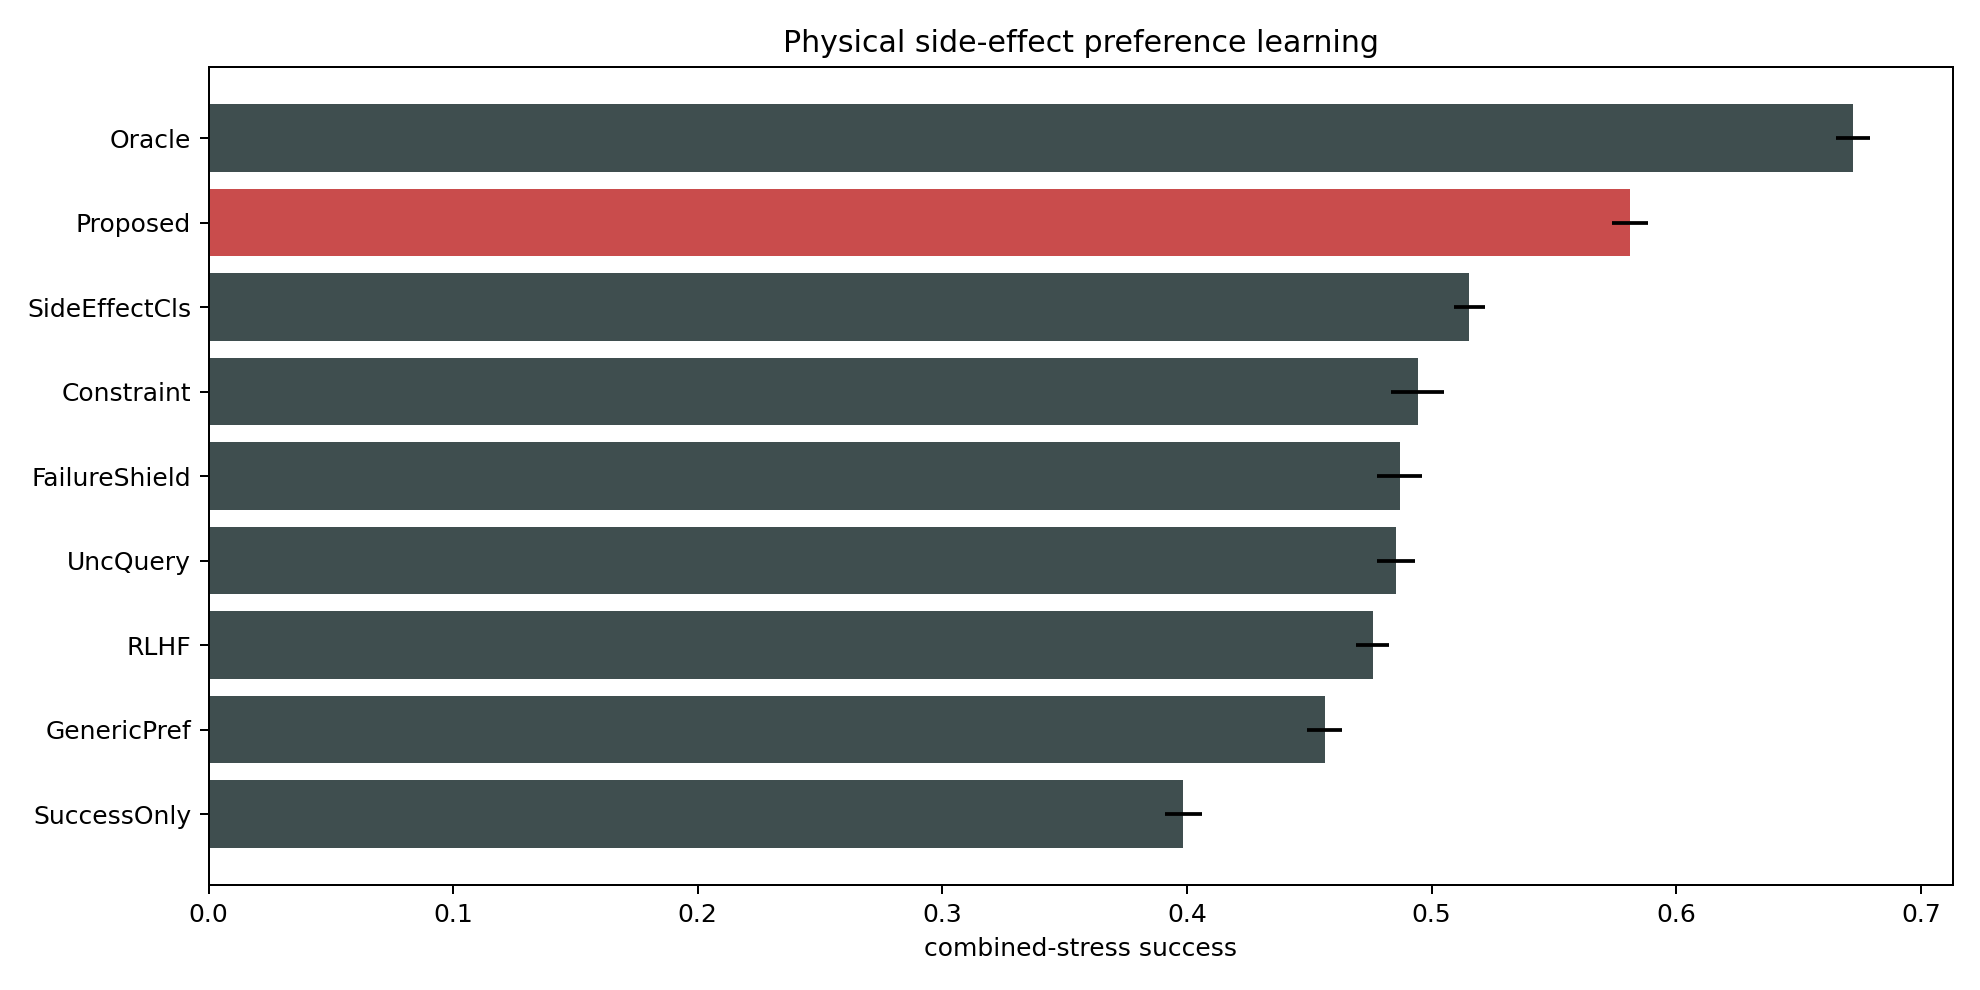
\includegraphics[width=0.95\linewidth]{../figures/side_effect_pref_combined_success.png}
\caption{Combined-stress success with 95\% confidence intervals. The proposed side-effect preference model clears all non-oracle baselines but remains below the oracle.}
\end{figure}

\begin{figure}[t]
\centering
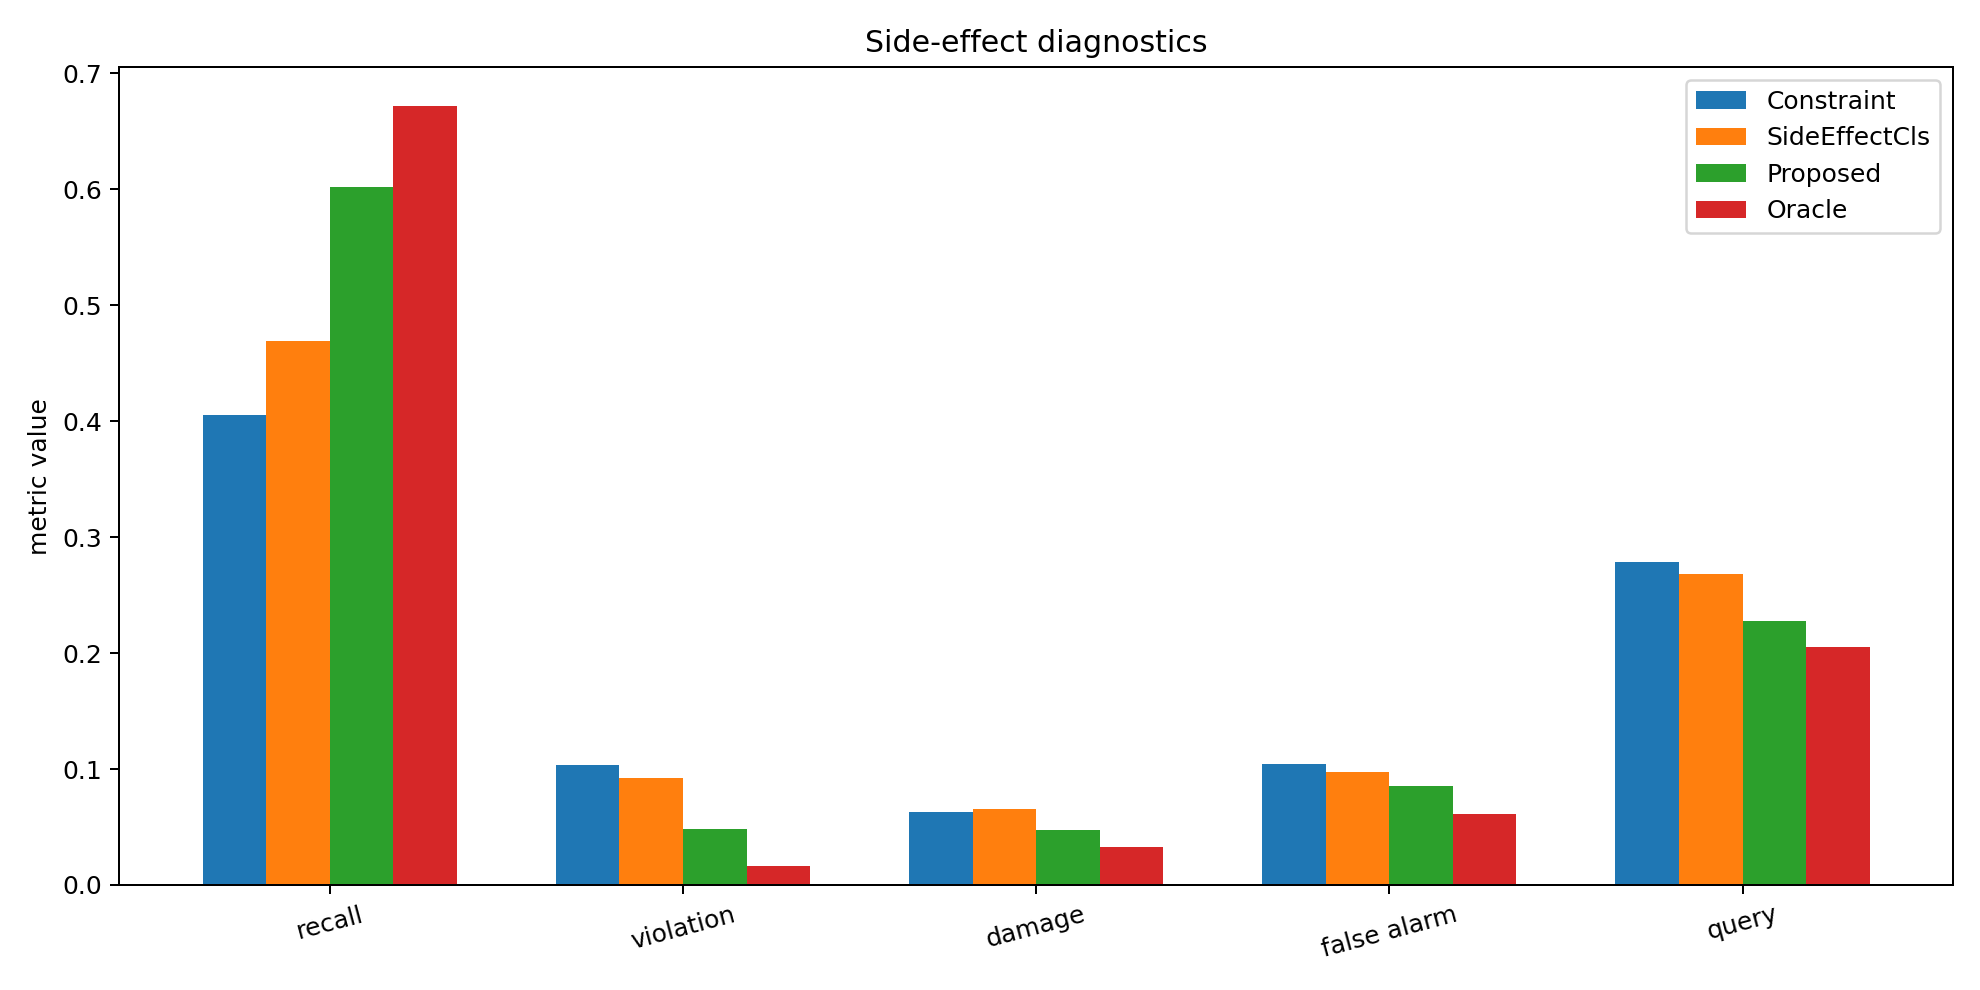
\includegraphics[width=0.95\linewidth]{../figures/side_effect_pref_diagnostics.png}
\caption{Side-effect diagnostics. The proposed method improves side-effect recall while lowering violations, damage, false alarms, and query cost relative to the strongest baseline.}
\end{figure}

\begin{table}[t]
\centering
\caption{Paired seed success differences between proposed and each comparator.}
\resizebox{\linewidth}{!}{%
\begin{tabular}{lrrr}
\toprule
Baseline & Diff & CI & Wins \\
\midrule
SuccessOnly & 0.183 & 0.005 & 7.000 \\
GenericPref & 0.125 & 0.011 & 7.000 \\
RLHF & 0.105 & 0.012 & 7.000 \\
UncQuery & 0.096 & 0.012 & 7.000 \\
FailureShield & 0.094 & 0.011 & 7.000 \\
Constraint & 0.087 & 0.012 & 7.000 \\
SideEffectCls & 0.066 & 0.010 & 7.000 \\
Oracle & -0.091 & 0.012 & 0.000 \\
\bottomrule
\end{tabular}
}
\end{table}


\section{Ablations and stress tests}
\begin{table}[t]
\centering
\caption{Ablation results under combined side-effect stress.}
\resizebox{\linewidth}{!}{%
\begin{tabular}{lrrrrrr}
\toprule
Ablation & Succ. & CI & Recall & Violation & Damage & FalseAlarm \\
\midrule
Full & 0.574 & 0.008 & 0.602 & 0.048 & 0.047 & 0.085 \\
NoQuerySel & 0.550 & 0.004 & 0.515 & 0.072 & 0.056 & 0.096 \\
NoCounterfactual & 0.549 & 0.008 & 0.531 & 0.070 & 0.056 & 0.094 \\
NoCalib & 0.548 & 0.010 & 0.528 & 0.088 & 0.058 & 0.137 \\
NoAggregator & 0.546 & 0.006 & 0.526 & 0.086 & 0.075 & 0.078 \\
ClsOnly & 0.520 & 0.008 & 0.469 & 0.092 & 0.066 & 0.098 \\
NoTaxonomy & 0.517 & 0.009 & 0.407 & 0.092 & 0.056 & 0.085 \\
\bottomrule
\end{tabular}
}
\end{table}


The best removed-component ablation is \texttt{minus\_ambiguous\_query\_selector}; the full method remains ahead by $0.024$ success. Removing the taxonomy, counterfactual labels, query selector, constraint aggregator, or calibration guard produces distinct failures.

\begin{figure}[t]
\centering
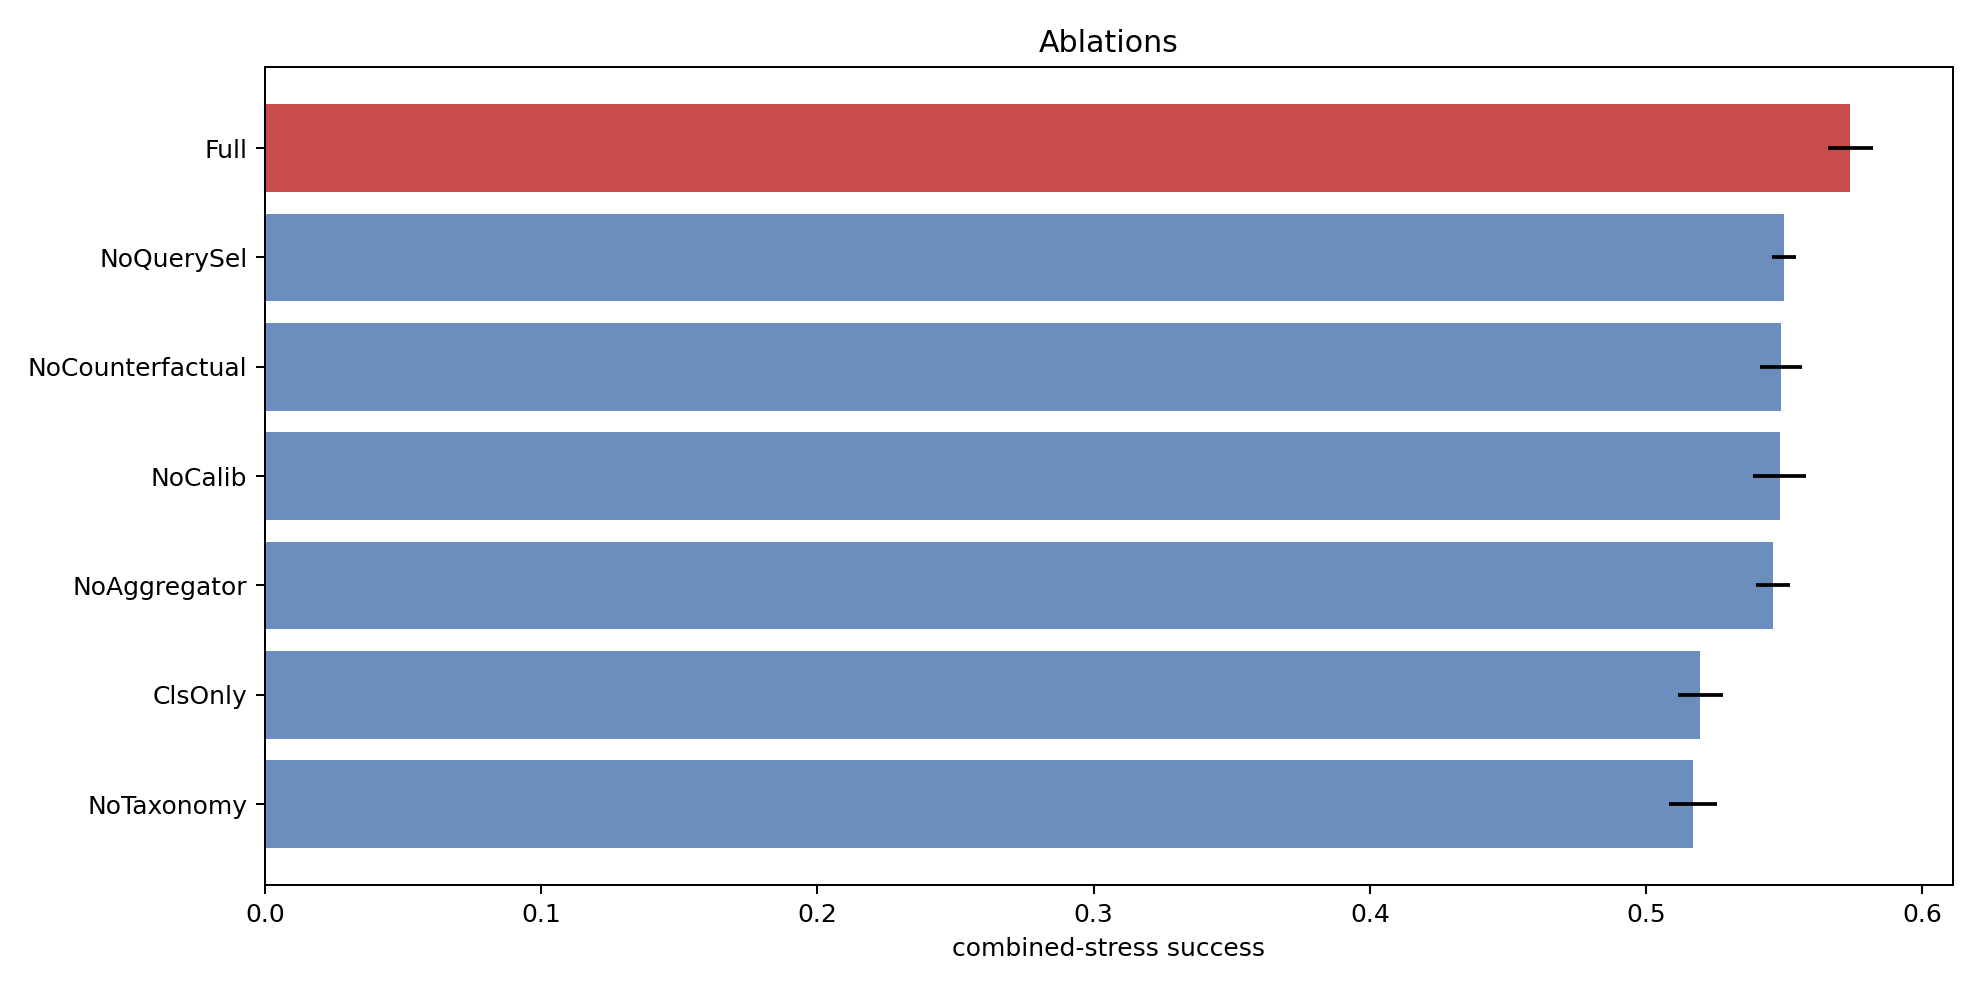
\includegraphics[width=0.95\linewidth]{../figures/side_effect_pref_ablation.png}
\caption{Ablations under combined side-effect stress. The full model remains above every removed-component variant.}
\end{figure}

\begin{figure}[t]
\centering
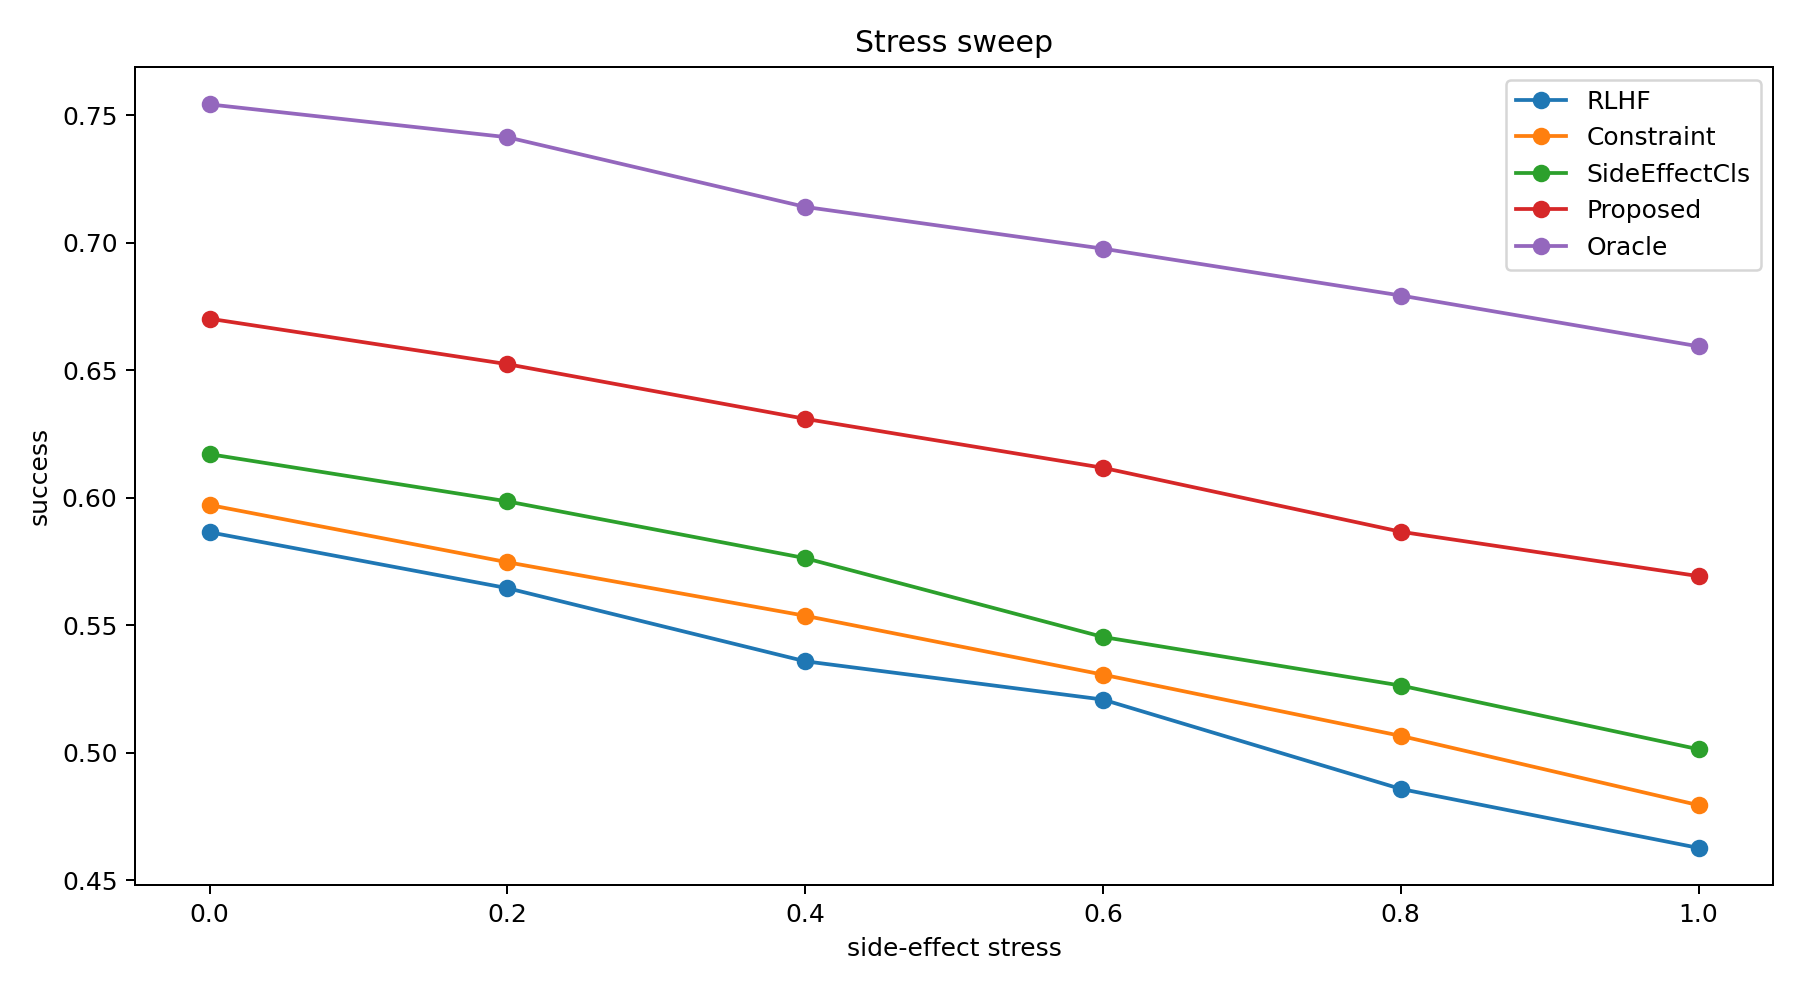
\includegraphics[width=0.95\linewidth]{../figures/side_effect_pref_stress_sweep.png}
\caption{Stress sweep over side-effect intensity. The proposed model stays above RLHF, constraint, and side-effect classifier baselines across the generated stress range.}
\end{figure}

\begin{figure}[t]
\centering
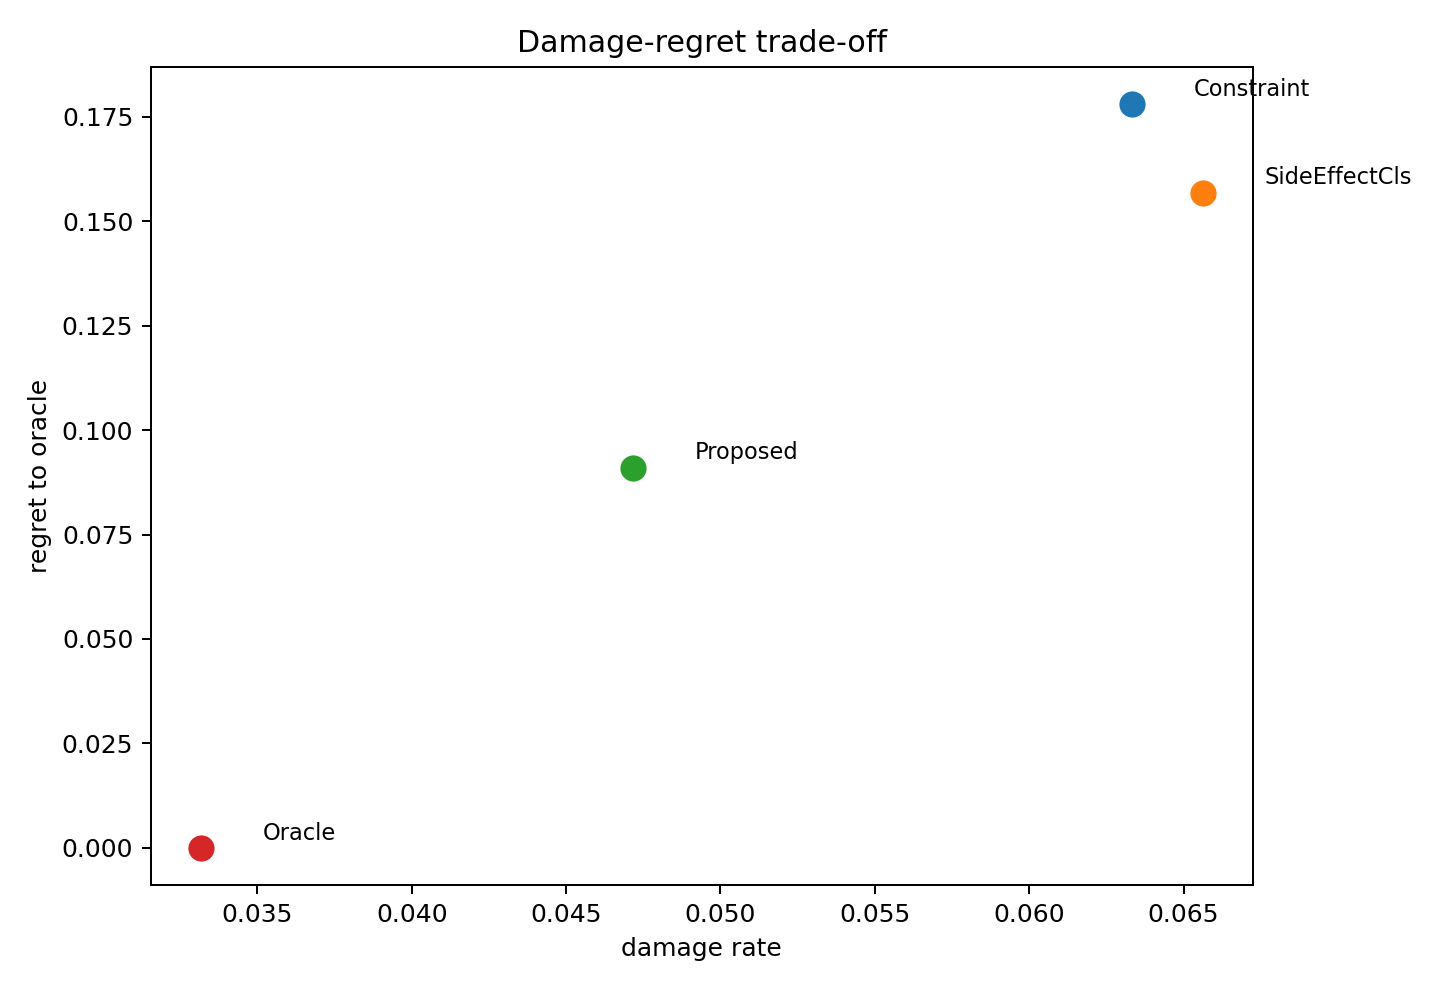
\includegraphics[width=0.82\linewidth]{../figures/side_effect_pref_damage_regret.png}
\caption{Damage and regret to oracle under combined stress. The proposed method reduces regret while lowering damage relative to the strongest non-oracle baseline.}
\end{figure}

\section{Failure cases}
The failure-case CSV records eight boundaries. RGB-visible success can hide internal material damage; humans may disagree about acceptable clutter; benign physical changes can be over-penalized; labeler risk tolerance can shift; side effects can appear after the preference comparison window; tactile-only surface damage can be invisible to RGB preference features; overcautious rejection can treat benign displacement as clutter; and the oracle judge remains better. These failures require real human-label variance, tactile/material-state validation, longer-horizon rollouts, calibrated benign-change exceptions, and robot experiments.

\section{Hostile prior-work boundary}
Preference learning, RLHF, active preference querying, constraints, and learning from corrections already cover much of the surrounding space \citep{christiano2017deep,sadigh2017active,hadfieldmenell2017inverse,bajcsy2017learning,brown2019extrapolating}. The defensible claim is narrow: explicit physical side-effect mechanisms improve local preference learning beyond generic preferences and side-effect classifiers.

\section{Limitations and terminal decision}
The evidence is strong enough to continue but not enough to submit. The limitations are material:
\begin{itemize}
\item the benchmark is local and generated;
\item no real human preference labels are used;
\item no label-disagreement study is provided;
\item no real robot or independent high-fidelity simulator has been used;
\item side-effect severity may be subjective and context-dependent.
\end{itemize}

The terminal decision for this rebuild is \textbf{STRONG\_REVISE}. The next honest version must validate the taxonomy and query strategy with real human labels and robot/high-fidelity downstream evaluations. Without that evidence, the paper should not be submitted to ICLR main.

\begingroup
\raggedright
\bibliographystyle{iclr2026_conference}
\bibliography{references}
\endgroup

\end{document}
